\section{Hybrid} \label{sec:hybrid_theory}
The hybrid approach consists of estimating the position using a \gls{lfp} method in combination with the \gls{pdr} algorithm. These algorithms of the hybrid solution can use each other to potentially achieve more accurate position estimations. Furthermore, hybrid solutions tend to achieve better performance, as described in \textbf{\autoref{sec:hybrid}}. The approach, which we have proposed, can be implemented in three ways, each presented in the following sections.

It should be noted that the \gls{pdr} algorithm cannot estimate the floor level. Therefore, for all hybrid solutions, the floor is estimated by the \gls{lfp} method alone.

A class diagram is presented in \textbf{\autoref{fig:hybrid_class_diagram}}. Since we will be working with multiple types of machine learning algorithms, a class for each machine learning algorithm is contained within \textit{ML Wrapper}. \textit{ML Wrapper} and \textit{PDR} are used to make up the three types of hybrid solutions, mentioned in this section.

\begin{figure}[H]
    \centering
    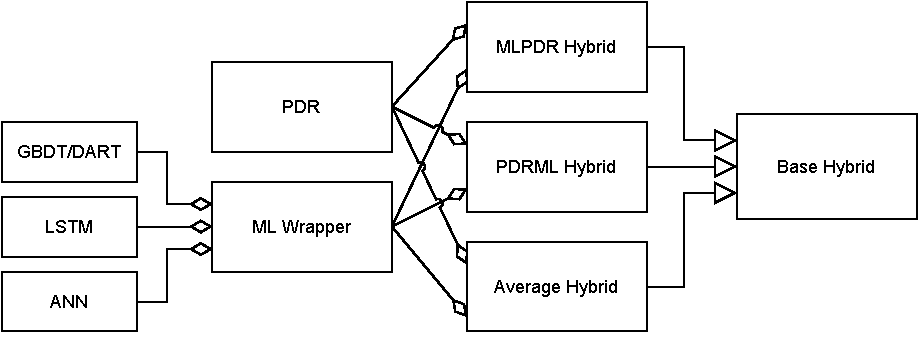
\includegraphics[scale=1]{Images/Experiments/hybrid/HybridClassDiagram.pdf}
    \caption{Class diagram of hybrid solution.}
     \label{fig:hybrid_class_diagram}
\end{figure}

\subsection{Location Fingerprinting as Primary and Pedestrian Dead Reckoning as Support}
This approach makes use of \gls{lfp} for positioning, where the \gls{pdr} algorithm is only used as support for whenever the \gls{lfp} method is not given any available \gls{rssi} data as input in a given period time. 
It happens that the \gls{lfp} method cannot determine a position if there are no \gls{rssi} values for the ground truth position. This approach idea is depicted in \textbf{\autoref{fig:hybrid1}}. In this case, \gls{pdr} will take over from the last know position estimated by \gls{lfp}.

\begin{figure}[H]
    \centering
    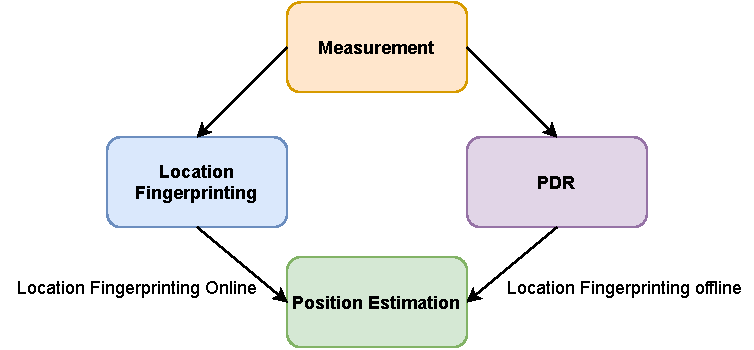
\includegraphics[scale=0.85]{Images/Experiments/hybrid/approach1.pdf}
    \caption{Hybrid solution using \gls{lfp} as primary and \gls{pdr} as support, where \textit{Location Fingerprinting} is offline when it is not able to make a position estimation given its input, and online when it is able to make a position estimation.}
     \label{fig:hybrid1}
\end{figure}

The performance of this hybrid option relies much on the performance of the \gls{lfp} method. \gls{pdr} will have no impact on the position estimations made by \gls{lfp}. However, as described, when there are no available \gls{rssi} data, \gls{pdr} will fill the missing position estimation. The less times it occurs that there is no available \gls{rssi} data, the more the performance of this hybrid option is alike the performance of the \gls{lfp} method alone. Described in \textbf{\autoref{alg:mlpdr_hybrid}}, the hybrid approach is shown, where \gls{lfp} is as primary and \gls{pdr} as support. 

% previous_wifi_data_timestamp er sidste timestamp, hvor LFP blev brugt.
% time_limit is a timeout time within which we need an estimation from LFP. If not, use PDR.
\begin{algorithm}[H]
\SetAlgoLined
\SetKw{KwIn}{in}
\SetKwInOut{Input}{Input}
\Input{$timestamp$, $\text{imu\_data}$ and $\text{wifi\_data}$}
\KwResult{($\text{x}$, $\text{y}$, $\text{floor}$)}
  $\text{lfp\_position}$ = $\text{lfp\_estimate\_position}$($\text{wifi\_data}$)\;
  
  \If{$timestamp - \text{previous\_wifi\_data\_timestamp} > \text{time\_limit} \lor \text{is\_empty}$($\text{wifi\_data}$)}{
      Re-calibrate \gls{pdr} to previous position estimation if \textit{if-statement} evaluated to false in previous position estimation\;
      $\text{pdr\_position}$ = $\text{pdr\_estimate\_position}$($\text{imu\_data}$)\;
      
      return $\text{pdr\_position}$\;
  }
  
  return $\text{lfp\_position}$\;
 \caption{Hybrid approach using \gls{lfp} as primary and \gls{pdr} as support.}
 \label{alg:mlpdr_hybrid}
\end{algorithm}

\subsection{Pedestrian Dead Reckoning as Primary and Location Fingerprinting as Support}
In this approach, the \gls{pdr} algorithm has the main responsibility at estimating positions. Although, as described in \textbf{\autoref{sec:IMUPositioning}}, \gls{pdr} drifts the more measurements it is given as input. Therefore, the \gls{lfp} method is needed to re-calibrate \gls{pdr} before it excessively drifts. The threshold value, $t$, for the number of measurements given as input is adjusted by experiments. This approach is depicted in \textbf{\autoref{fig:hybrid2}}.

\begin{figure}[H]
    \centering
    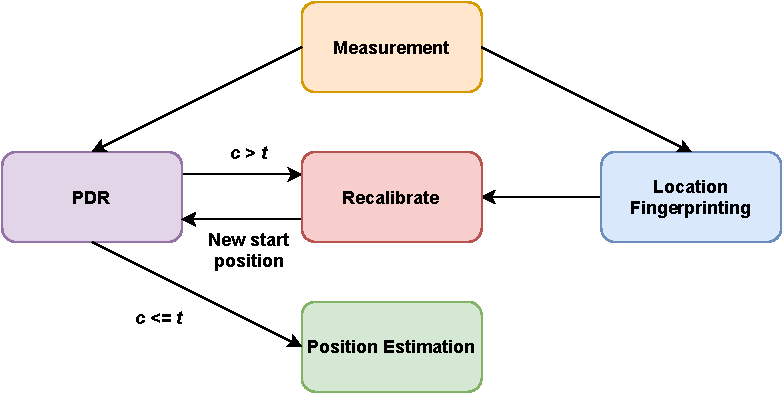
\includegraphics[scale=0.85]{Images/Experiments/hybrid/approach2.pdf}
    \caption{Hybrid solution using \gls{pdr} as primary and \gls{lfp} as support, where $c$ is measurement count and $t$ is a threshold value for measurement count.}
     \label{fig:hybrid2}
\end{figure}

This option aims at improving the accuracy of the experiments of \gls{pdr} by re-calibrating \gls{pdr} at fixed points in time. The re-calibration is accomplished using the position estimation from \gls{lfp}, which makes the overall accuracy dependent on the accuracy of \gls{lfp} at re-calibration time.
Since the odds of a position estimation of the \gls{lfp} method is far off the ground truth is low, the \gls{pdr} method should have the optimal environment for estimating positions. Since the \gls{pdr} is re-calibrated at fixed points in time, \gls{pdr} should not deviate excessively from the ground truth path. Therefore, this hybrid option should yield better results compared to the \gls{pdr} experiments because of its re-calibration, as we have noted during the \gls{pdr} experiments that it is accurate for fewer \gls{imu} measurements. The algorithm for this hybrid method is shown in \textbf{\autoref{alg:pdrml_hybrid}}.

% recalibration_limit er en konstant for antallet af estimeringer før PDR skal gen-kalibreres.
\begin{algorithm}[H]
\SetAlgoLined
\SetKw{KwIn}{in}
\SetKwInOut{Input}{Input}
\Input{$timestamp$, $\text{imu\_data}$ and $\text{wifi\_data}$}
\KwResult{($\text{x}$, $\text{y}$, $\text{floor}$)}
  $\text{pdr\_position}$ = $\text{pdr\_estimate\_position}$($\text{imu\_data}$)\;
  $\text{lfp\_position}$ = $\text{lfp\_estimate\_position}$($\text{wifi\_data}$)\;
  $\text{measurement\_count}$ = $\text{measurement\_count} + 1$\;
  
  \If{$\text{measurement\_count} \geq \text{recalibration\_limit}$}{
      Re-calibrate \gls{pdr} to position estimation of \gls{lfp}\;
  }
  
  return ($\text{pdr\_position.get\_x}$(), $\text{pdr\_position.get\_y}$(), $\text{lfp\_position}.get\_floor$())\;
 \caption{Hybrid approach using \gls{pdr} as primary and \gls{lfp} as support.}
 \label{alg:pdrml_hybrid}
\end{algorithm}

\subsection{Average Between Location Fingerprinting and Pedestrian Dead Reckoning Outputs}
This approach makes use of both the \gls{lfp} and \gls{pdr} algorithms, actively. This approach estimates the position by taking the average position estimation from \gls{lfp} and \gls{pdr}. \gls{pdr} is re-calibrated after a fixed number of measurements are given as input, where this number is estimated from experiments. This approach is illustrated in \textbf{\autoref{fig:hybrid3}}

\begin{figure}[H]
    \centering
    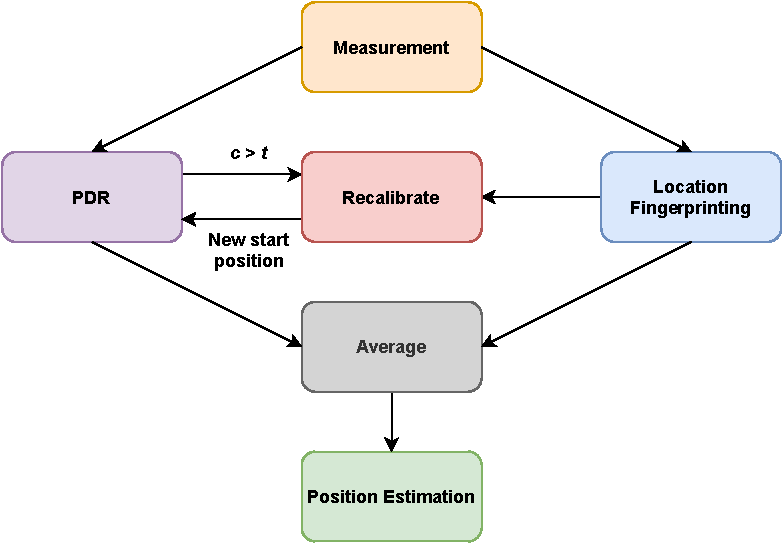
\includegraphics[scale=0.85]{Images/Experiments/hybrid/approach3.pdf}
    \caption{Hybrid solution using the average position estimation from \gls{pdr} and \gls{lfp}, where $c$ is measurement count and $t$ is a fixed threshold value for measurement count.}
     \label{fig:hybrid3}
\end{figure}

It is possible that any of \gls{lfp} and \gls{pdr} estimate a position that is not close to the ground truth position at any position estimation. Therefore, if one of \gls{lfp} and \gls{pdr} is accurate and the other is not, the other will drag its position estimation away from the ground truth. This is a problem since \gls{pdr} is known to drift the more measurements it is given as input. However, it is also possible the \gls{lfp} method will make a position estimation that is far off the ground truth position.
Thereby, using the average between the position estimation of both \gls{lfp} and \gls{pdr} will decrease the impact of the inaccurate position estimation made by any of \gls{lfp} and \gls{pdr}, separately. The approach of this method is explained in pseudo code in \textbf{\autoref{alg:average_hybrid}}.
The main motivation for this approach is that if both position estimation methods are accurate but each of them deviate a bit from the ground truth, then it is possible to achieve a better estimation by considering the estimations from both approaches.

% estimation_count er antallet af nuværende estimeringer.
% recalibration_limit er en konstant for antallet af estimeringer før PDR skal gen-kalibreres.
\begin{algorithm}[H]
\SetAlgoLined
\SetKw{KwIn}{in}
\SetKwInOut{Input}{Input}
\Input{$timestamp$, $\text{imu\_data}$ and $\text{wifi\_data}$}
\KwResult{($\text{x}$, $\text{y}$, $\text{floor}$)}
 $\text{lfp\_position}$ = $\text{lfp\_estimate\_position}$($\text{wifi\_data}$)\;
 $\text{pdr\_position}$ = $\text{pdr\_estimate\_position}$($\text{imu\_data}$)\;
 $\text{avg\_x}$ = $\text{pdr\_position}.get\_x$()\;
 $\text{avg\_y}$ = $\text{pdr\_position}.get\_y$()\;
 
 \If{$\text{lfp\_position}$ $\neq$ $\text{null}$}{
     $\text{avg\_x}$ = ($\text{avg\_x}$ + $\text{lfp\_position}.get\_x$()) / 2\;
     $\text{avg\_x}$ = ($\text{avg\_y}$ + $\text{lfp\_position}.get\_y$()) / 2\;
     
     \If{$\text{estimation\_count > recalibration\_limit}$}{
         Re-calibrate \gls{pdr} to position estimation of \gls{lfp}\;
     }
     
 return ($\text{avg\_x}$, $\text{avg\_x}$, $\text{lfp\_position}.get\_floor$())
 }
 \caption{Hybrid approach using average between \gls{lfp} and \gls{pdr} for position estimation.}
 \label{alg:average_hybrid}
\end{algorithm}